\problemname{Kebab Pizza}

Alice loves pizza and plans to throw a pizza party for her birthday, where she will make one big, round pizza for all her guests.
She knows that her friends are a bit special when it comes to pizza:
Julie does not want any vegetables but loves kebab meat on her pizza.
Katy would never eat pizza with cheese on top.
Alice herself is a huge fan of pineapple on pizza, while Mickey absolutely hates it.
Instead, he wants to put spaghetti on it, which everybody else finds weird.
The list goes on and on.
Briefly put, it is absolutely impossible to accommodate everybody.

As a compromise, Alice decides to let each person choose two toppings for their pizza slice in advance.
Each person will be happy if their slice has exactly their two chosen toppings and none of the others.
Note that a person may choose the same topping twice, in which case they just get twice the amount of that topping.

\begin{figure}[!h]
	\centering
	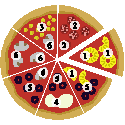
\includegraphics[width=0.4\textwidth]{sample.pdf}
	\caption{Illustration of Sample Input 1, with two toppings numbered on
	every slice in one possible solution. Note that each topping only occurs
	on a single range of pizza slices.}
    \label{fig:k}
\end{figure}

On the day of her party, Alice discovers that the rolled out pizza dough takes up so much space on her kitchen counter that she can only prepare one kind of topping at a time.
To optimise the workflow and to make sure that the pizza is ready in time for
her party, she wants to take out each chosen kind of topping only once and then add it
on a consecutive range of pizza slices.
Note that the whole pizza forms a consecutive range of pizza slices in a circular fashion.
Determine whether it is possible to prepare the pizza in this way while satisfying all the chosen topping combinations.
See Figure~\ref{fig:k} for an example.

\begin{Input}
    The input consists of:
    \begin{itemize}
        \item One line with two integers $n$ and $k$ ($3\leq n, k \leq 10^5$), the number of pizza slices and the number of possible toppings which are numbered from $1$ to $k$.
        \item $n$ lines, each with two integers $a$ and $b$ ($1\leq a, b \leq k$), describing the toppings chosen by the $i$th person.
    \end{itemize}
\end{Input}

\begin{Output}
    Output ``\texttt{possible}'' if it is possible for Alice to select a
    consecutive range of pizza slices for each chosen topping such that the
    resulting pizza can be split into $n$ suitable slices.
    Otherwise, output ``\texttt{impossible}''.
\end{Output}
